\documentclass[11pt,border=2pt]{standalone}
\usepackage{amsmath,amssymb}
\usepackage{xcolor}
\usepackage{tikz}
\usepackage{pgfplots}
\pgfplotsset{compat=1.18}
\usetikzlibrary{calc,arrows,positioning,fit,backgrounds,decorations.pathreplacing,patterns}
\definecolor{cElem}{RGB}{40,80,140}
\definecolor{cTrg}{RGB}{190,40,40}
\definecolor{cCell}{RGB}{225,238,248}
\definecolor{cAcc}{RGB}{240,200,120}
\definecolor{cGrey}{RGB}{120,120,120}
\definecolor{cVec}{RGB}{110,55,150}
\begin{document}
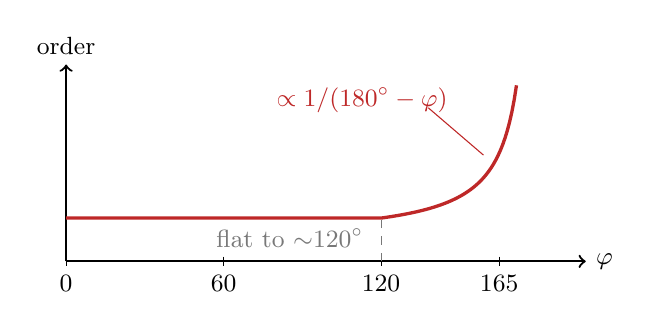
\begin{tikzpicture}[scale=1.0]
  \draw[->,thick] (0,0) -- (6.6,0) node[right,font=\small] {$\varphi$};
  \draw[->,thick] (0,0) -- (0,2.5) node[above,font=\small] {order};
  \foreach \x/\l in {0/0,2/60,4/120,5.5/165} \draw (\x,0.06)--(\x,-0.06) node[below,font=\small] {\l};
  \draw[cTrg,very thick] (0,0.55) -- (4,0.55)
        plot[domain=4:5.72,samples=60] (\x,{0.55+0.55/(6.0-\x)-0.55/2.0});
  \node[cTrg,font=\small,anchor=west] at (2.55,2.05) {$\propto 1/(180^\circ-\varphi)$};
  \draw[cTrg,thin] (4.6,1.95) -- (5.3,1.35);
  \draw[dashed,cGrey] (4,0)--(4,0.55);
  \node[cGrey,font=\small,anchor=east] at (3.9,0.30) {flat to $\sim$120$^\circ$};
\end{tikzpicture}
\end{document}
